% =====================================================================
%  9. PROJECT DESIGN
% =====================================================================
\section{Project Design}\label{sec:design}

This section presents the planned system architecture, the front-end prototype of \projectname{}, and how the design applies recognised usability principles. The design follows the project's research focus (Section~\ref{sec:rqs}): the interface is meant not only to display predictions, but to help moderators review accounts accurately, efficiently and with an appropriate level of trust in the model.


\subsection{System Overview}\label{sec:system-overview}

\projectname{} integrates a data pipeline, a machine learning model layer, an API and a front end into a single architecture (Figure~\ref{fig:architecture}).

\begin{figure}[htbp]
\centering
\begin{tikzpicture}[
    node distance=0.6cm,
    tierbox/.style={draw=brandprimary, fill=brandprimary!6, rounded corners=3pt, align=left,
                  font=\footnotesize\sffamily, text width=2.35cm, minimum height=3.3cm},
    actor/.style={draw=brandaccent, fill=brandaccent!8, rounded corners=3pt, align=center,
                  font=\footnotesize\sffamily, text width=1.5cm, minimum height=3.3cm},
    arrow/.style={-{Stealth[length=2.2mm]}, thick, brandprimary!80},
    both/.style={{Stealth[length=2.2mm]}-{Stealth[length=2.2mm]}, thick, brandprimary!80},
    stage/.style={font=\scriptsize\sffamily, text=brandmuted}
]
  \node[tierbox] (data) {\textbf{Data pipeline}\\[2pt]Labelled account data\\Cleaning and pre-processing\\PRISMO feature selection (GA, PSO, SA)};
  \node[tierbox, right=of data] (model) {\textbf{Model layer}\\[2pt]Four classifiers\\10-fold cross-validation\\Model selection and export};
  \node[tierbox, right=of model] (api) {\textbf{API (FastAPI)}\\[2pt]Single and batch prediction\\Explanations\\Review logging\\Validation and errors};
  \node[tierbox, right=of api] (fe) {\textbf{Front end (React.js)}\\[2pt]Dashboard\\Check account\\Batch triage\\Insights and charts};
  \node[actor, right=of fe] (user) {\textbf{Moderator}\\[2pt]Reviews and decides};

  \draw[arrow] (data) -- (model);
  \draw[arrow] (model) -- (api);
  \draw[both] (api) -- (fe);
  \draw[both] (fe) -- (user);

  \node[stage, below=0.15cm of data] {Offline, Stage 2};
  \node[stage, below=0.15cm of model] {Offline, Stage 2};
  \node[stage, below=0.15cm of api] {Runtime, Stage 3};
  \node[stage, below=0.15cm of fe] {Runtime, Stage 3};
\end{tikzpicture}
\caption{System architecture of \projectname{}}
\label{fig:architecture}
\end{figure}

\begin{itemize}[nosep]
  \item \textbf{Data pipeline.} Prepares the labelled account data, then applies feature preparation and PRISMO's two-layer feature selection (Section~\ref{sec:prismo}).
  \item \textbf{Model layer.} Trains and compares Random Forest, Na\"ive Bayes, a rule-based learner and a decision tree, then exports the best-performing model together with its pre-processing and feature-selection steps.
  \item \textbf{API (FastAPI).} Loads the exported model and provides endpoints for single-account checks, batch triage, explanations and moderator reviews, with input validation and error handling. Because the same pre-processing is used for training and prediction, results in the application are consistent with the evaluated model (R10).
  \item \textbf{Front end (React.js).} Provides moderators with a dashboard, input forms, batch triage tools and interactive visualisations (built with a library such as Plotly.js), communicating with the API through JSON over HTTP.
\end{itemize}

Table~\ref{tab:api} lists the planned API endpoints. They use both the GET and POST methods required by the unit and correspond directly to actions in the prototype.

\begin{table}[htbp]
\centering
\caption{Planned API endpoints}
\label{tab:api}
\begin{tabularx}{\textwidth}{@{}l >{\raggedright\arraybackslash}p{0.25\textwidth} >{\raggedright\arraybackslash}X l@{}}
  \toprule
  \textbf{Method} & \textbf{Endpoint} & \textbf{Purpose} & \textbf{Req.} \\
  \midrule
  GET  & \texttt{/api/features} & Names, units and valid ranges of the selected features; drives manual input and its validation & FR15, FR18 \\
  GET  & \texttt{/api/samples} & Sample accounts for the \emph{Sample Account} selector & FR15 \\
  POST & \texttt{/api/predict} & Score one account; returns the label, spam score, review flag and explanation & FR11--FR13 \\
  POST & \texttt{/api/batches} & Validate an uploaded batch and score every account & FR16, FR18 \\
  POST & \texttt{/api/reviews} & Save a moderator's decision and notes, keeping the original prediction unchanged & FR21, FR23 \\
  GET  & \texttt{/api/batches/\{id\}/export} & Export predictions, decisions and review notes as CSV & FR16 \\
  GET  & \texttt{/api/metrics} & Model evaluation and feature selection results for the insights page & FR14, FR19 \\
  \bottomrule
\end{tabularx}
\end{table}

\subsection{Front-end Prototype}\label{sec:prototype}

The front-end prototype was designed in Figma by \memberFour{} as a clickable prototype with interactions. It uses illustrative data throughout, which is marked by a \emph{Demo mode} badge and a footer reminding users that data is illustrative and human review is required. Every screen shares the same layout: a navy sidebar with four workspace areas (Dashboard, Check account, Batch triage and Insights), a breadcrumb, and a consistent colour code of red for \emph{likely spam}, amber for \emph{needs review} and teal for \emph{likely genuine}.
\href{https://www.figma.com/design/4Z7n5mLQY9oHJUmVBQmA1i/SpamSentinel?node-id=1-2&t=1zb9kp3R3MiX9RbX-1}{(Click to view SpamSentinel Figma prototype)}

The prototype follows a moderator's workflow from start to finish. The moderator signs in to the workspace and lands on the dashboard. From there, they check a single account or load a batch, inspect the explanation for a flagged account, record a review decision, and export the results. Figures~\ref{fig:proto-login}--\ref{fig:proto-mobile} show the main desktop screens and the mobile view.

\paragraph{Sign-in (Figure~\ref{fig:proto-login}).} The entry screen introduces \projectname{} as a \emph{moderator workspace}, with an example account card that previews what the tool does: a spam score and the signals behind it. The prototype also shows a \emph{Sign Up} button, but self-registration will not be implemented. Account registration and stored user accounts remain out of scope (Table~\ref{tab:in-out-scope}).

\begin{figure}[htbp]
\centering
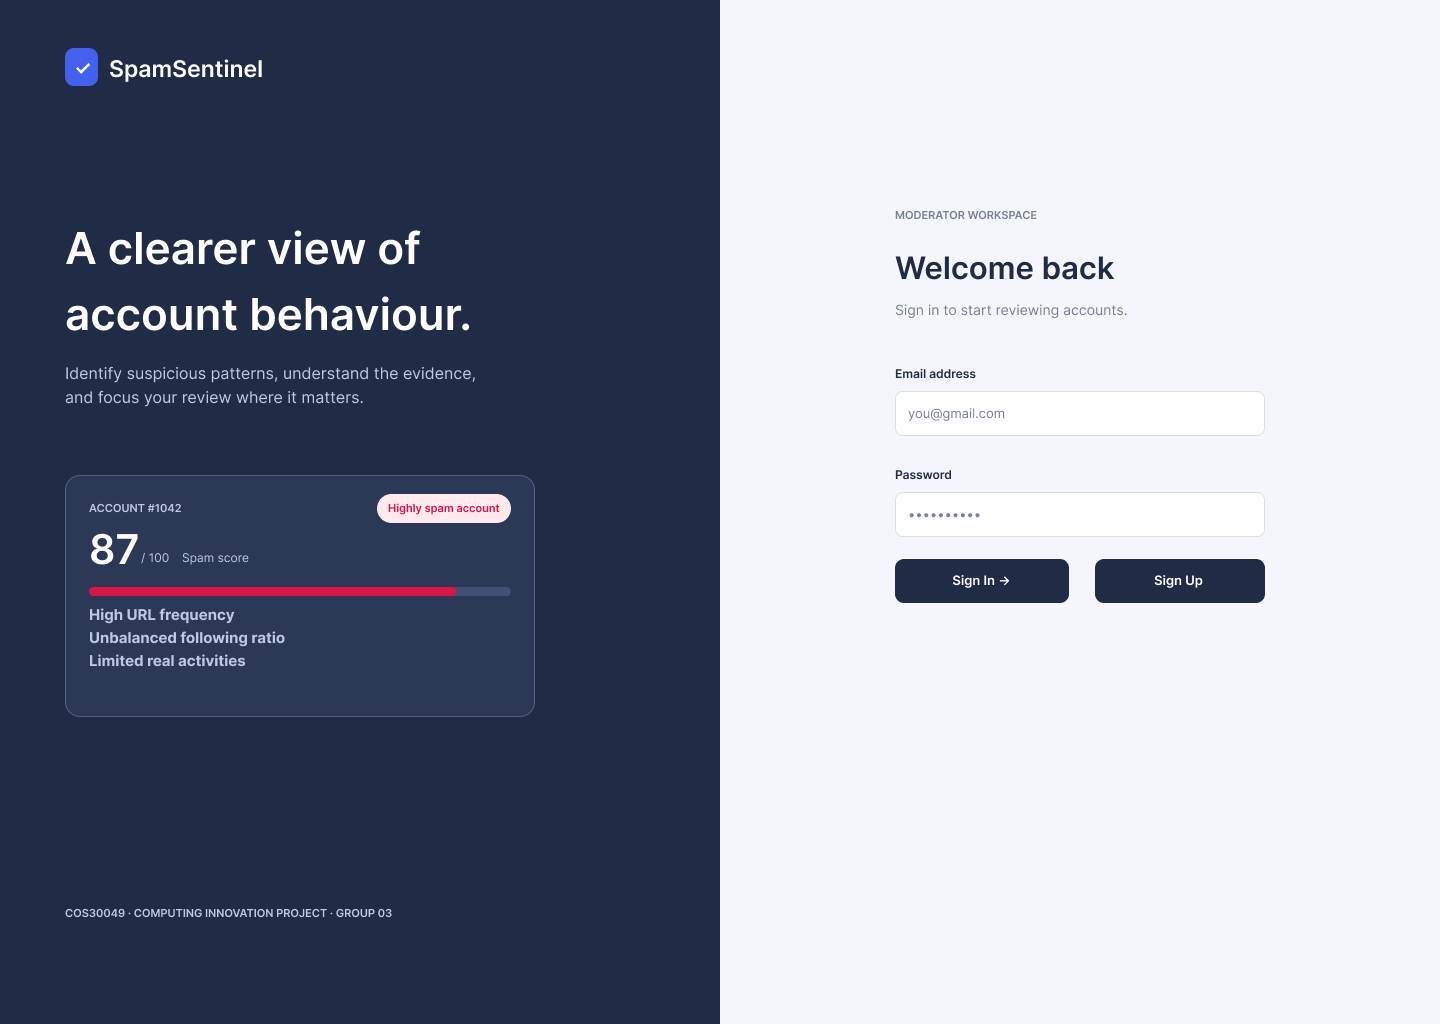
\includegraphics[width=0.92\textwidth]{proto-login}
\caption{Prototype: sign-in screen for the moderator workspace}
\label{fig:proto-login}
\end{figure}

\paragraph{Dashboard (Figure~\ref{fig:proto-dashboard}).} The \emph{Account review overview} summarises the current batch in four cards (accounts analysed, likely spam, needs review and likely genuine). It shows the distribution of spam scores in a histogram, tracks review progress, and lists a priority review queue. Two shortcuts start the main tasks: \emph{Check an Account} and \emph{Upload Account Batch}. The note \enquote{Model predictions stay separate from your decisions} reinforces that the moderator, not the model, makes the final call (FR16, FR19).

\begin{figure}[htbp]
\centering
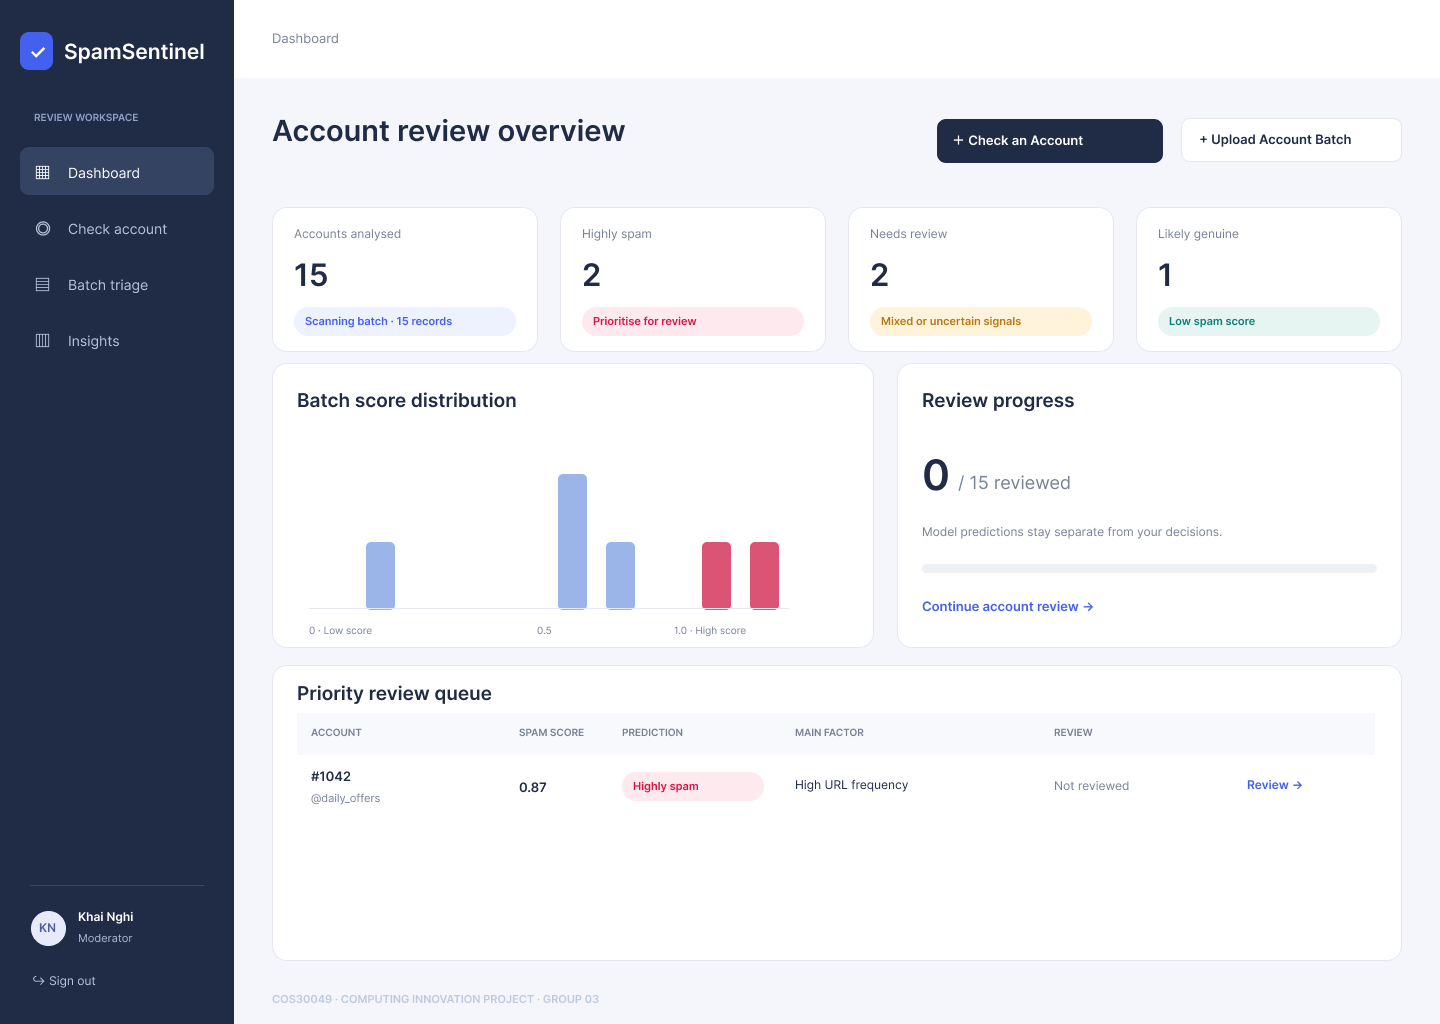
\includegraphics[width=0.92\textwidth]{proto-dashboard}
\caption{Prototype: dashboard with summary cards, score distribution, review progress and priority queue}
\label{fig:proto-dashboard}
\end{figure}

\paragraph{Single account check (Figure~\ref{fig:proto-check}).} Moderators can choose a sample account or switch to the \emph{Input Account Information} tab to enter feature values manually (FR15). A feature preview shows the key values before analysis. The result panel then presents the prediction label, the spam score with a score bar, and the three key signals to review, in plain language (FR12). From the result, the moderator can open the full explanation or record a review. Before an account is analysed, an empty state explains what to do next (\enquote{Ready to analyse}).

\begin{figure}[htbp]
\centering
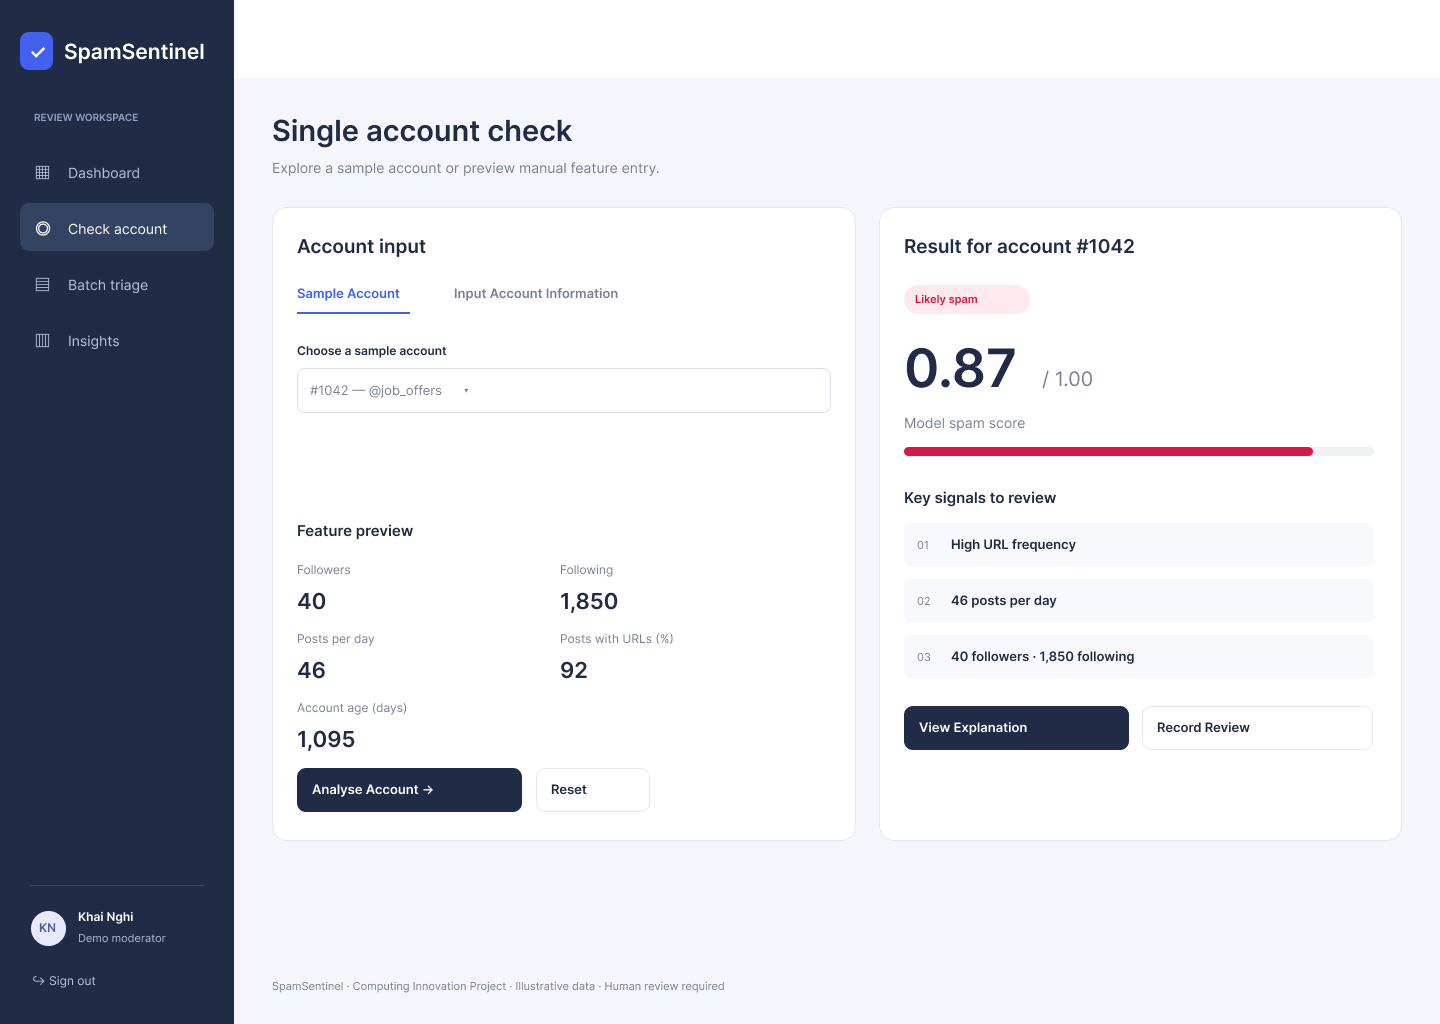
\includegraphics[width=0.92\textwidth]{proto-check}
\caption{Prototype: single account check with feature preview, spam score and key signals}
\label{fig:proto-check}
\end{figure}

\paragraph{Batch triage (Figure~\ref{fig:proto-batch}).} A batch is processed in three steps: load the accounts, validate the features (required columns and numeric values), and review the predictions. The account review queue is sorted by spam score and shows each account's prediction, main factor and review status. It can be searched and filtered by prediction. Moderators can start a new batch, clear filters, and export the predictions together with their decisions and review notes (FR16, FR18).

\begin{figure}[htbp]
\centering
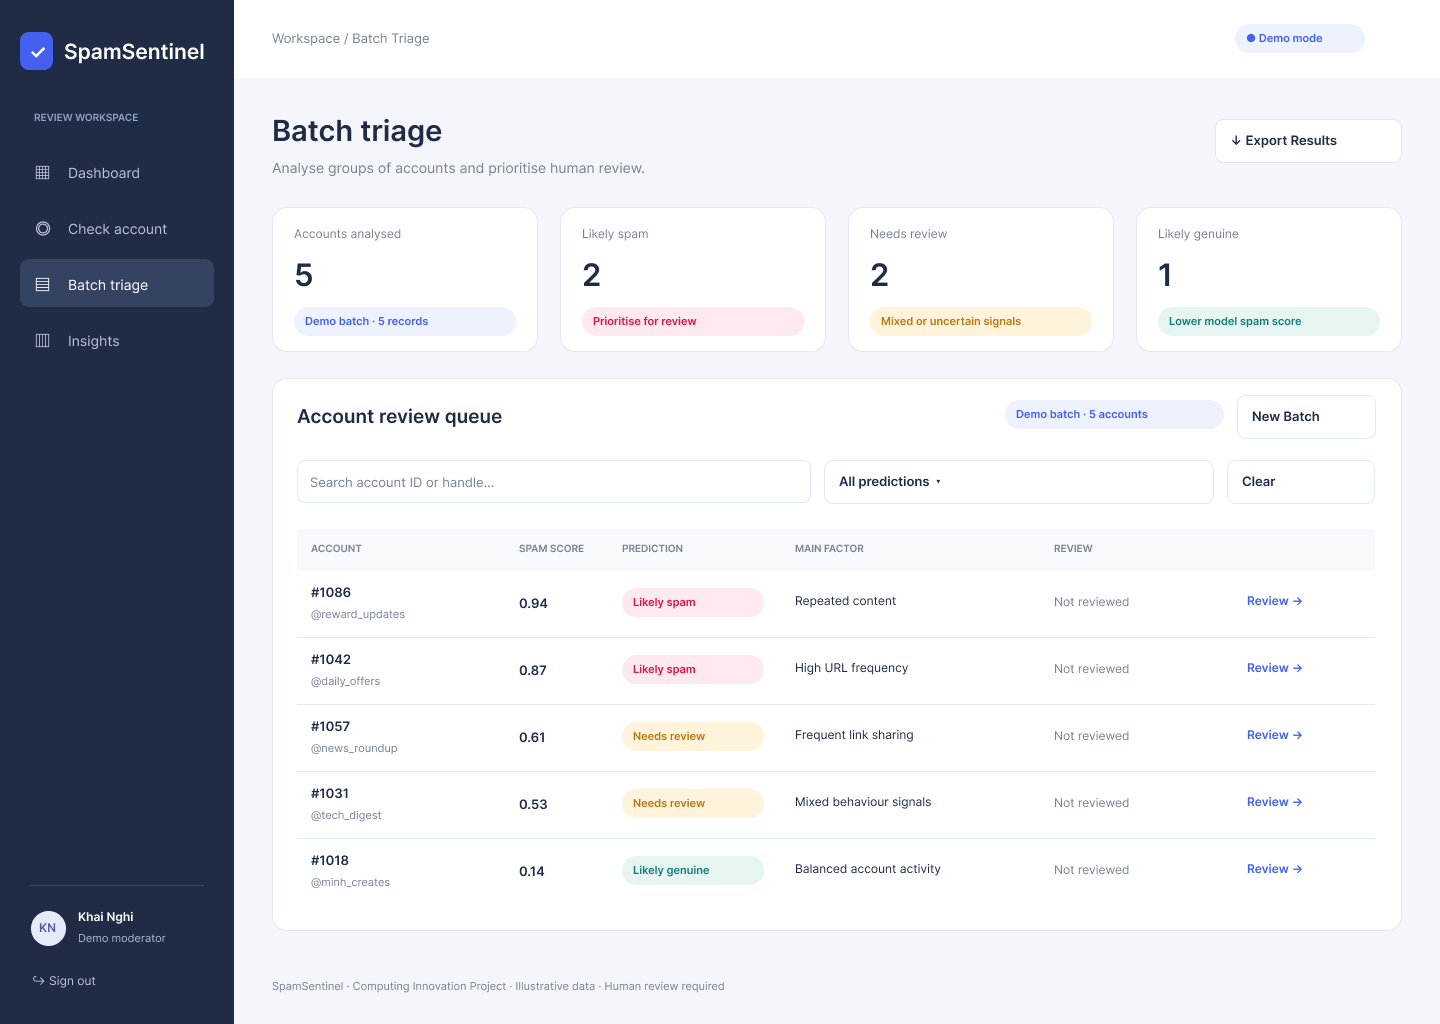
\includegraphics[width=0.92\textwidth]{proto-batch}
\caption{Prototype: batch triage queue sorted by spam score, with search, filtering and export}
\label{fig:proto-batch}
\end{figure}

\paragraph{Human review panel (Figure~\ref{fig:proto-review}).} Selecting \emph{Review} opens a side panel with the account's prediction, spam score and main factor, a link to the full explanation, a decision selector and a field for review notes (FR21). After the review is saved, the queue confirms \enquote{Review recorded for account \#1042. Original prediction preserved}, and the row's status changes to \emph{Reviewed}. Keeping the model's prediction separate from the moderator's decision also makes it possible to measure how often users override the model, which is central to RQ4 (FR23).

\begin{figure}[htbp]
\centering
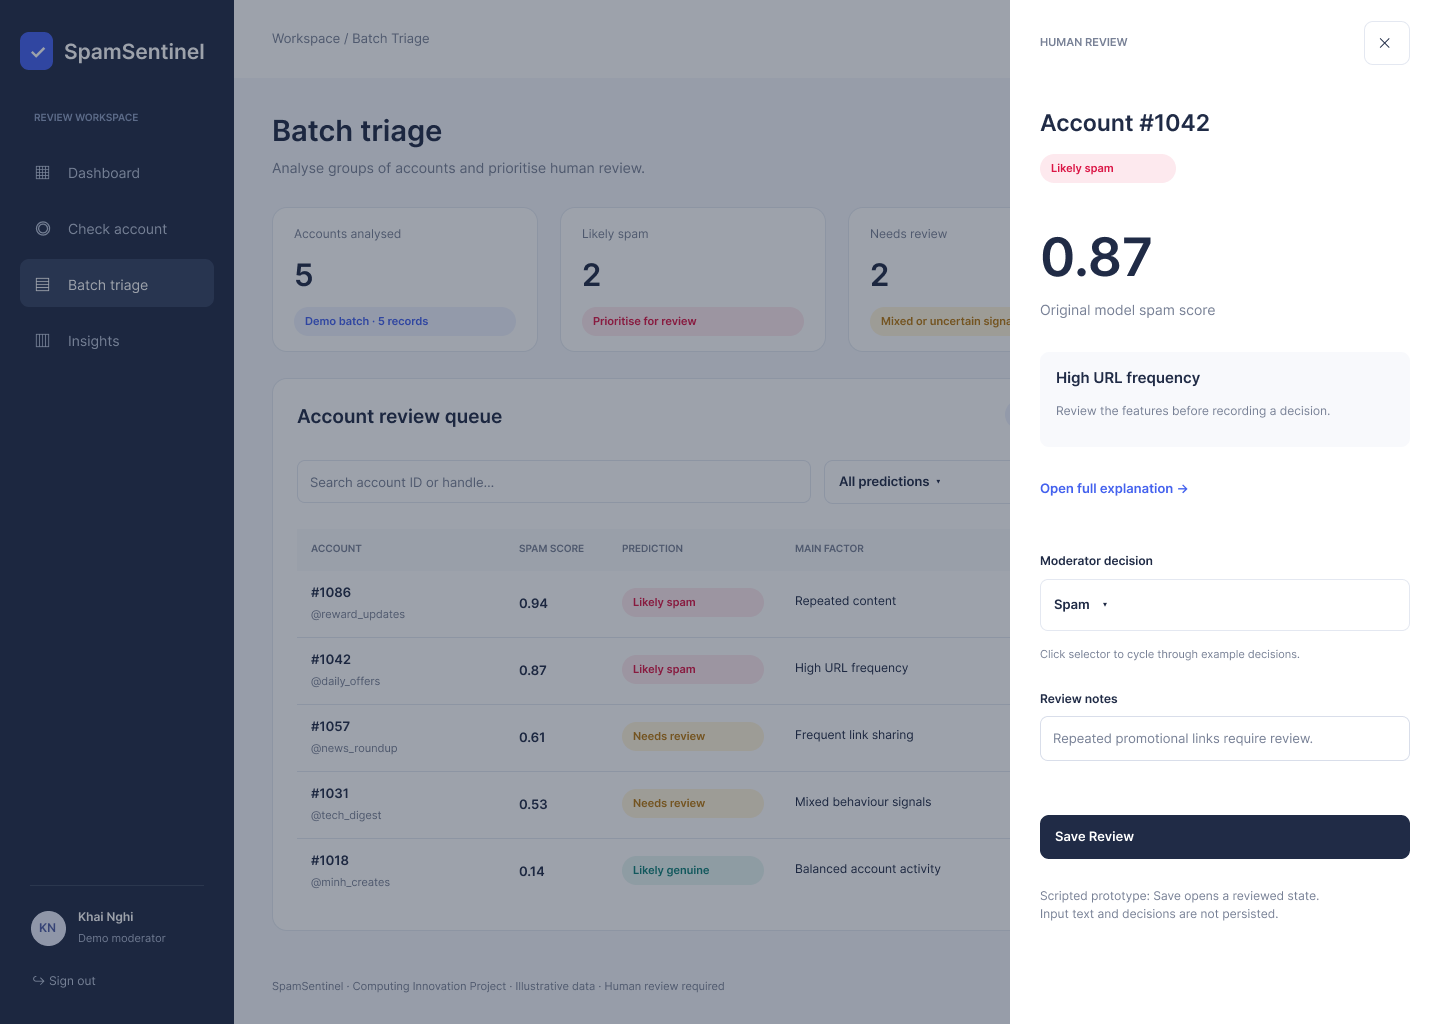
\includegraphics[width=0.92\textwidth]{proto-review}
\caption{Prototype: human review panel for recording a moderator decision and notes}
\label{fig:proto-review}
\end{figure}

\paragraph{Account explanation (Figure~\ref{fig:proto-explanation}).} The \emph{Explanation \& insights} page shows why an account received its score. A contribution chart shows how much each feature increased (red) or decreased (teal) the score, with details available on hover (FR11, FR19). Alongside it, \emph{feature evidence} cards explain each factor in plain language and compare it with a genuine-account reference, for example \enquote{92\% of posts contain URLs \ldots\ genuine reference: under 20\%} (FR12). A note confirms that raw posts, comments and private messages are not included, reflecting the project's privacy requirement (NFR10).

\begin{figure}[htbp]
\centering
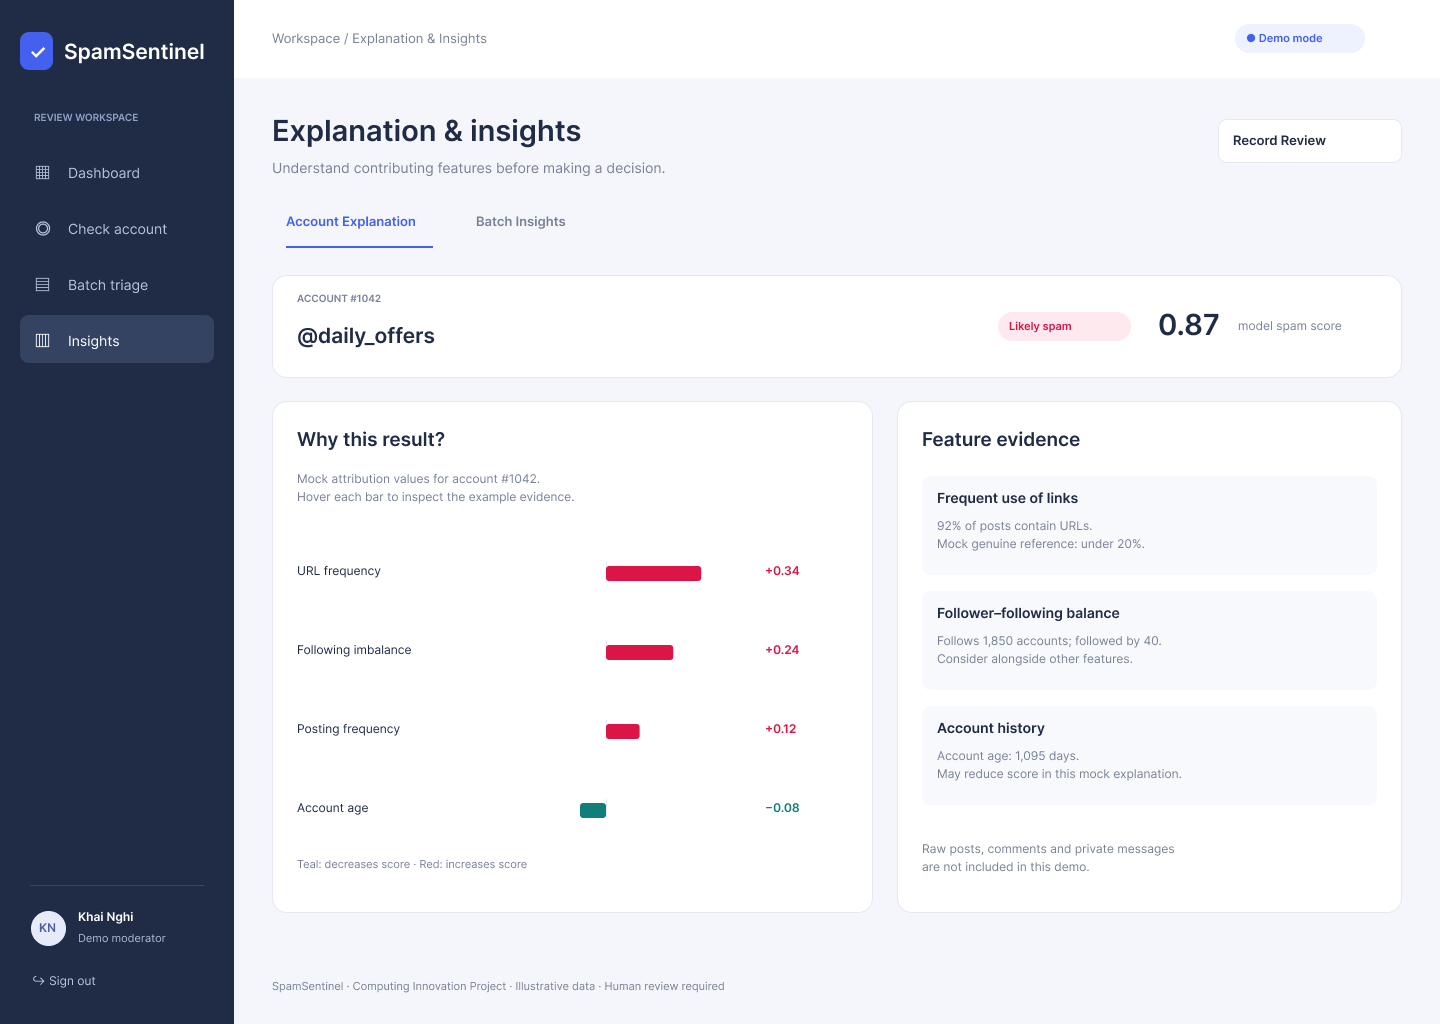
\includegraphics[width=0.92\textwidth]{proto-explanation}
\caption{Prototype: account explanation with feature contribution chart and plain-language feature evidence}
\label{fig:proto-explanation}
\end{figure}

\paragraph{Batch insights (Figure~\ref{fig:proto-insights}).} The \emph{Batch Insights} tab shows the score distribution of the current batch as an interactive histogram. The \emph{Model evaluation} panel is deliberately left as a placeholder (\enquote{Awaiting experimental results}): no performance values are claimed until the experiments in Stage~2 are complete. After Assignment~2, this panel will compare precision, recall and F1-score across classifiers and feature sets (FR9, FR14).

\begin{figure}[htbp]
\centering
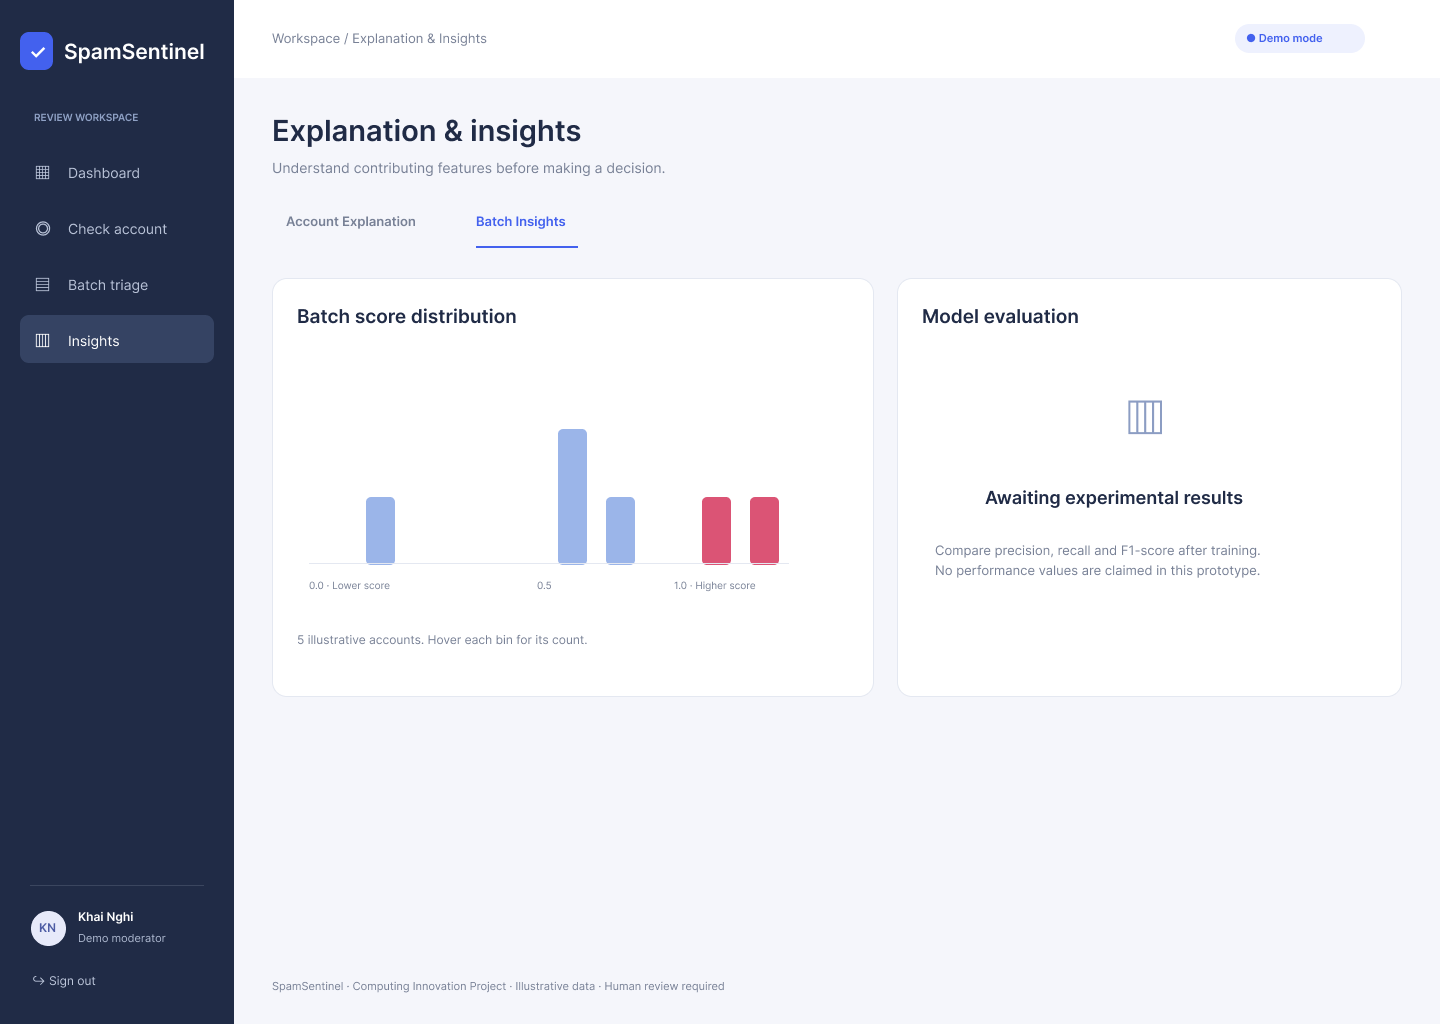
\includegraphics[width=0.92\textwidth]{proto-insights}
\caption{Prototype: batch insights with score distribution and the model evaluation panel awaiting results}
\label{fig:proto-insights}
\end{figure}

\paragraph{Mobile view (Figure~\ref{fig:proto-mobile}).} The mobile prototype adapts the same workflow to a phone screen, using the same colours, badges and wording as the desktop design (NFR7):

\begin{itemize}[nosep]
  \item \textbf{Navigation.} The sidebar is replaced by a bottom tab bar (Dashboard, Check, Batch and Insights), which keeps the four workspace areas within thumb reach.
  \item \textbf{Layout.} Cards stack in a single column and the summary cards form a two-by-two grid.
  \item \textbf{Touch targets.} Primary actions become full-width buttons.
  \item \textbf{Account result.} The score bar marks the uncertainty \emph{review zone} directly (FR13), so users can see how close an account is to needing human review.
  \item \textbf{Review sheet.} Recording a review opens a bottom sheet over the queue, with a three-way decision control (Spam, Genuine or Escalate), review notes, and a reminder that the original model prediction is kept alongside the moderator's decision (FR21).
\end{itemize}

\begin{figure}[htbp]
\centering
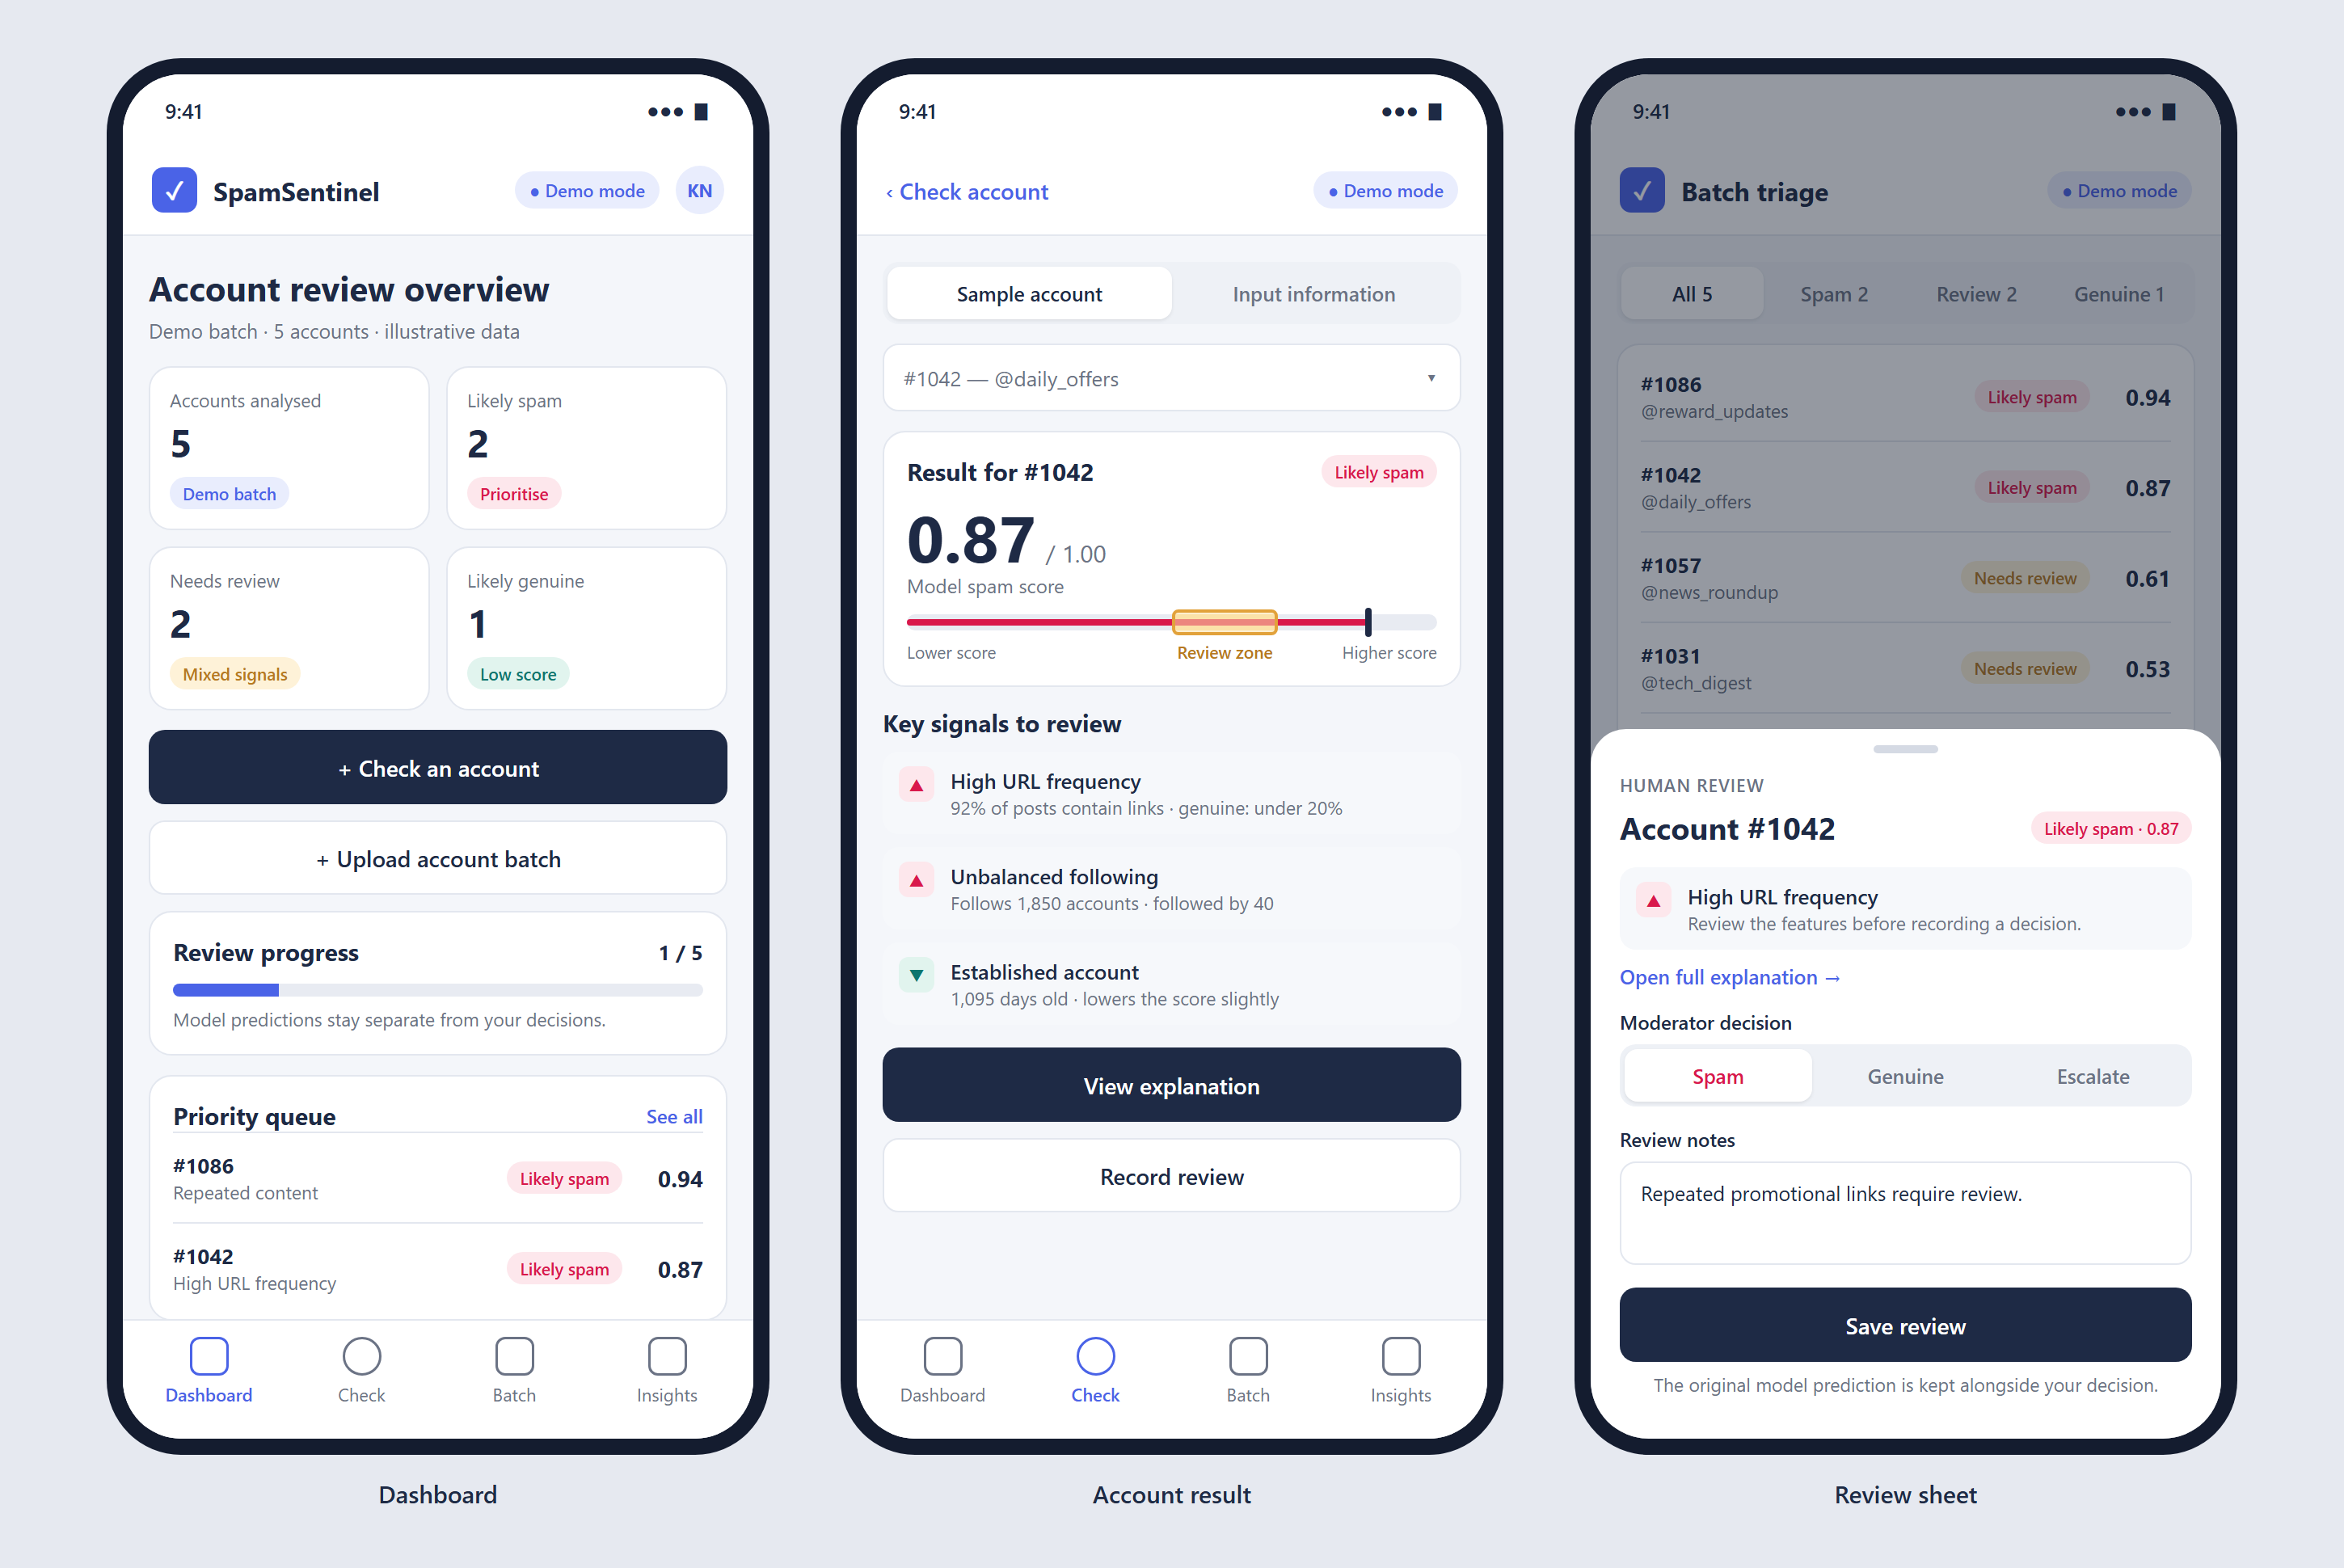
\includegraphics[width=\textwidth]{proto-mobile}
\caption{Prototype: mobile view of the dashboard, account result and human review sheet}
\label{fig:proto-mobile}
\end{figure}

\paragraph{Planned refinements.} The prototype will be refined before milestone M6 (Section~\ref{sec:milestones}) based on a heuristic review by the team:

\begin{itemize}[nosep]
  \item design the manual input form for the selected features, with units, valid ranges and field-level error messages (FR15, FR18);
  \item bring the review zone shown on the mobile score bar into the desktop design, so that users can see why an account needs review (FR13);
  \item add the model evaluation chart once results are available, giving at least three interactive chart types (FR19);
  \item design tablet layouts and mobile versions of the explanation and insights screens (NFR7); and
  \item use the same label wording (e.g.\ \emph{Likely spam}) on every screen.
\end{itemize}

\subsection{Alignment with Usability Principles}\label{sec:usability}

The design follows Nielsen's ten usability heuristics \parencite{nielsen1994heuristics}. It offers clear system feedback, plain-language explanations and consistent layouts. Moderators keep control through review and override options, and errors are prevented through validation and uncertainty warnings. Table~\ref{tab:heuristics} shows how each heuristic is applied in the prototype.

{\renewcommand{\arraystretch}{1.2}\small
\begin{longtable}{@{}>{\raggedright\arraybackslash}p{0.22\textwidth} >{\raggedright\arraybackslash}p{0.58\textwidth} >{\raggedright\arraybackslash}p{0.12\textwidth}@{}}
  \caption{Application of Nielsen's usability heuristics in the prototype}\label{tab:heuristics} \\
  \toprule
  \textbf{Heuristic} & \textbf{How the Design Applies It} & \textbf{Figures} \\
  \midrule
  \endfirsthead
  \multicolumn{3}{@{}l}{\small\itshape Table~\thetable{} continued} \\
  \toprule
  \textbf{Heuristic} & \textbf{How the Design Applies It} & \textbf{Figures} \\
  \midrule
  \endhead
  \bottomrule
  \endlastfoot
  1. Visibility of system status & A step indicator shows progress through batch processing; review progress (\enquote{0 / 15 reviewed}) and each account's review status are always visible; saving a review produces an immediate confirmation; filtered views state how many accounts are shown. & \ref{fig:proto-dashboard}, \ref{fig:proto-batch}, \ref{fig:proto-review} \\
  2. Match between system and the real world & Factors are described in plain language (\enquote{High URL frequency}, \enquote{Follows 1,850 accounts; followed by 40}) and compared with genuine-account references; categories and actions use moderators' own vocabulary: likely spam, needs review, review notes. & \ref{fig:proto-check}, \ref{fig:proto-explanation} \\
  3. User control and freedom & Moderators can reset inputs, clear filters, start a new batch, close panels and dialogs, and change or override the model's prediction, while the original prediction is preserved. & \ref{fig:proto-batch}, \ref{fig:proto-review} \\
  4. Consistency and standards & The sidebar, breadcrumb, footer, card style and colour-coded badges are identical on every screen, so the same prediction looks the same wherever it appears. & All \\
  5. Error prevention & Sample accounts avoid manual-entry mistakes; batches are validated for required columns and numeric values before analysis; a separate \emph{needs review} category avoids forcing uncertain cases into a label. & \ref{fig:proto-check}, \ref{fig:proto-batch} \\
  6. Recognition rather than recall & Each queue row shows its main factor; key signals appear next to the score; evidence cards sit beside the chart; decisions are chosen from a selector rather than typed. & \ref{fig:proto-check}, \ref{fig:proto-review}, \ref{fig:proto-explanation} \\
  7. Flexibility and efficiency of use & Dashboard shortcuts start the two main tasks; the queue is sorted by spam score so the riskiest accounts come first; search, filters and export speed up work on large batches. & \ref{fig:proto-dashboard}, \ref{fig:proto-batch} \\
  8. Aesthetic and minimalist design & Only the three key signals are shown by default, with full detail one click away; each panel has a single primary action; no model performance figures are shown until real results exist. & \ref{fig:proto-check}, \ref{fig:proto-insights} \\
  9. Help users recognise, diagnose and recover from errors & Batch validation reports missing columns or non-numeric values before analysis; an empty filtered view explains how to restore all results; manual input will show field-level messages explaining how to correct each value. & \ref{fig:proto-batch} \\
  10. Help and documentation & Page subtitles explain each screen's purpose; chart legends explain colours (\enquote{Teal: decreases score · Red: increases score}); hover details and inline guidance (\enquote{Review the features before recording a decision}) support users at the point of need. & \ref{fig:proto-review}, \ref{fig:proto-explanation} \\
\end{longtable}
}

\paragraph{Designing for appropriate trust.} Because \projectname{} supports human decisions, the design aims to make users trust the model only as much as it deserves. Explanations let moderators check each prediction against the evidence. The \emph{needs review} category signals when the model is unsure. Messages such as \enquote{Human review required} and \enquote{Original prediction preserved} make clear that the model advises rather than decides. Whether these choices improve decision accuracy and reduce over-reliance is tested directly by RQ3 and RQ4.

\paragraph{Accessibility and responsiveness.} Prediction categories are always shown as text labels, not by colour alone, and colours will be checked against WCAG 2.1 Level AA contrast guidelines \parencite{w3c2018wcag21}. The React implementation will use a responsive layout for desktop, tablet and mobile screens, following the mobile prototype in Figure~\ref{fig:proto-mobile} (NFR6, NFR7).

\paragraph{Evaluation of the design.} The team will carry out a heuristic evaluation of the refined prototype against Table~\ref{tab:heuristics} before M6. The finished application will then be evaluated with users in the study, using task time, decision accuracy and the System Usability Scale \parencite{brooke1996sus}, against the target of a score of at least 68 (NFR4).
